% cas-consensus-protocol.tex

\documentclass{standalone}

\usepackage{tikz}
\usetikzlibrary{shapes, positioning, arrows.meta, backgrounds, fit}

\begin{document}
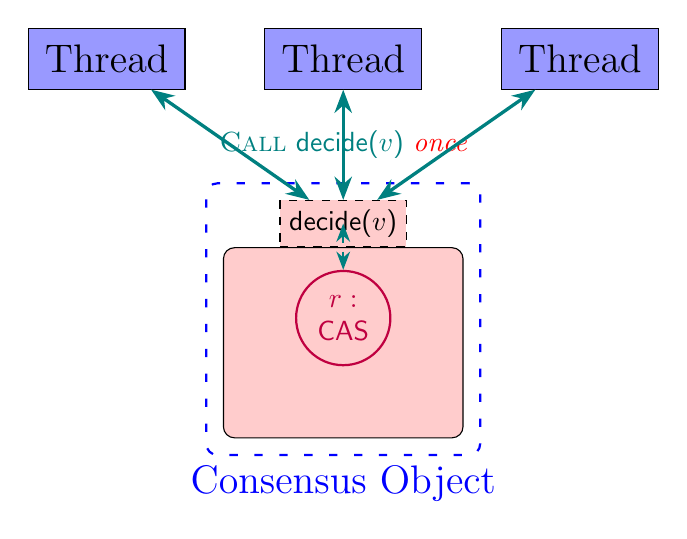
\begin{tikzpicture}[thread/.style = {draw, rectangle, fill = blue!40, font = \Large, inner sep = 6pt},
    call/.style = {>=Stealth, <->, very thick, teal},
    incall/.style = {>=Stealth, <->, thick, dashed, teal},
    cas/.style = {draw, circle, thick, purple, minimum size = 5pt, align = center},
    rw/.style = {draw, ellipse, thick, cyan, font = \footnotesize},]
  \node (cas1) [cas] {$r: $ \\ \textsf{CAS}};
  \node (cas2) [cas, draw = none, below left = 0.50cm and 0.50cm of cas1] {};
  \node (cas3) [cas, draw = none, below right = 0.50cm and 0.50cm of cas1] {};

  % \node (rw1) [rw, left = 0.20cm of cas1] {R/W};
  % \node (rw2) [rw, right = 0.20cm of cas1] {R/W};

  \begin{pgfonlayer}{background}
    \node (so) [draw, rectangle, rounded corners, fit = (cas1) (cas2) (cas3),
	  font = \large, fill = red!20, align = center, inner sep = 8pt] {};
  \end{pgfonlayer}
  \node (decide) [draw, rectangle, above = 0.0cm of so, dashed, fill = red!20] {\textsf{decide($v$)}};

  \node (tm) [thread, above = 2.0cm of so] {Thread};
  \node (tl) [thread, left = of tm] {Thread};
  \node (tr) [thread, right = of tm] {Thread};

  \draw [call] (tm) to node [] {\textsf{\textsc{Call} decide($v$)} \textcolor{red}{\it once}} (decide);
  \draw [call] (tl) to (decide);
  \draw [call] (tr) to (decide);

  \draw [incall] (decide.center) to (cas1);
  % \draw [incall] (decide.center) to (cas2);
  % \draw [incall] (decide.center) to (cas3);
  % \draw [incall, cyan] (decide.center) to (rw1);
  % \draw [incall, cyan] (decide.center) to (rw2);
  
  \begin{pgfonlayer}{background}
    \node (consensus-cas) [draw, thick, blue, rectangle, rounded corners, loosely dashed, fit = (so) (decide), inner sep = 6pt,
	label = {[font = \Large, align = center, blue]-90:{Consensus Object}}] {};
  \end{pgfonlayer}
\end{tikzpicture}
\end{document}